\section{Περιγραφή Λειτουργίας Μετατροπέας Υποβιβασμού}

\subsection{Μετατροπέας υποβιβασμού}

\noindent
Ο Μετασχηματιστής Υποβιβασμού είναι μία συσκευή η οποία δέχεται στην είσοδο της μία Dc τάση και ένα Dc ρεύμα και δίνει στην έξοδό της μία Dc τάση και ένα Dc ρεύμα χαμηλότερου επιπέδου.  Για την κατασκευή του χρησιμοποιείται ένας ελεγχόμενος ηλεκτρικός διακόπτης, μία δίοδο ισχύος, ένα πηνίο και έναν πυκνωτή στην εξής συνδεσμολογία:
\begin{figure}[h]
	\centering
	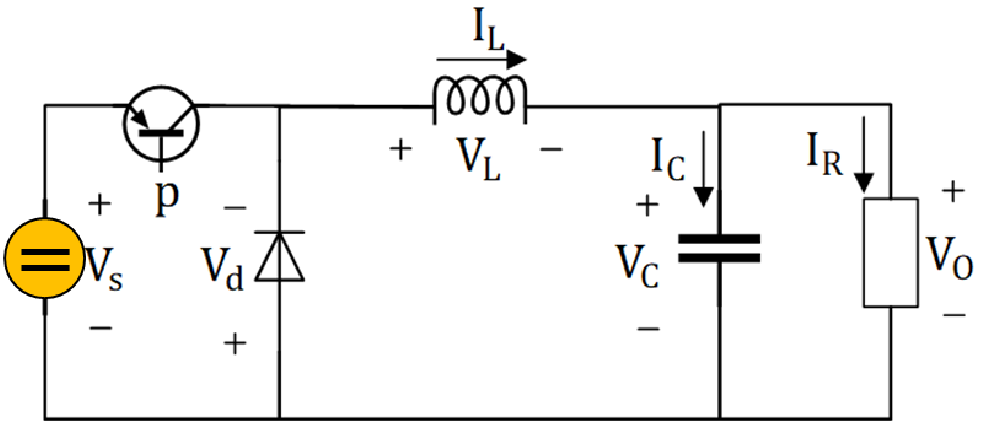
\includegraphics[width=0.4\textwidth]{Images/buckConverter.png}
\end{figure}

\noindent
Ο διακόπτης παραμένει κλειστός για χρόνο ίσο με $D \cdot T$ και για το διάστημα αυτό, η τάση εξόδου ισούται με την τάση εισόδου, ενώ για το υπόλοιπο διάστημα παραμένει ανοιχτός και η τάση εξόδου ισούται με 0. Επίσης, δεδομένης της πολύ μεγάλης διακοπτικής συχνότητας, το φορτίο αντιλαμβάνεται την μέση τιμή της $V_o$ η οποία υπολογίζεται ως εξής:
\begin{equation}
	\bar{V_o} = \frac{1}{T} \int_{0}^{T} V_o(t) dt = \frac{1}{T} \int_{0}^{D\cdot T} V_s dt = V_s \cdot D	
\end{equation} 

δηλαδή ορίζοντας την τιμή του Duty Cycle κατάλληλα, μπορεί να ελεγχθεί το επίπεδο της τάσης εξόδου.

\noindent\\
Όσον αφορά τα υπόλοιπα στοιχεία του κυκλώματος, η δίοδος είναι εκεί διότι, το πηνίο χρησιμοποιείται για την σταθεροποίηση του ρεύματος και ο πυκνωτής για την σταθεροποίηση της τάσης.
\subsubsection{Κλειστός Διακόπτης (Φ1)}
\label{Phase_1}
\noindent
Κατά την φάση Φ1, εφαρμόζοντας κατάλληλη τιμή τάσης στον διακόπτη οπότε κλειστός (βραχυκύκλωμα). Ως αποτέλεσμα, η δίοδος ανακυκλώνεται καθώς είναι ανάστροφα πολωμένη εφόσον στην άνοδό της πηγής συνδέεται το αρνητικό άκρο της πηγής και στην κάθοδο το θετικό. 

\begin{figure}[h]
	\centering
	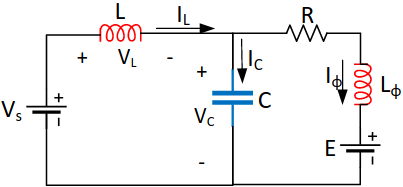
\includegraphics[width=0.35\textwidth]{Images/Phase_1}
\end{figure}

\noindent
Για την επίλυση του συστήματος είναι απαραίτητο να οριστούν οι μεταβλητές εισόδου και εξόδου.  Ως μεταβλητές εισόδου ορίζονται η τάση εισόδου ($V_s$) και η τάση ($E$) ενώ ως μεταβλητές εισόδου ορίζονται τα ρεύματα των πηνίων ($I_L$, $Ι_{\Phi}$) και η τάση του πυκνωτή ($V_C$). Επιπλέον, είναι απαραίτητο να βρεθούν οι πίνακες A, B, C και D:
\begin{align}
	\dot{X} = A\cdot X + B\cdot U \label{x_dot}\\
	Y = C \cdot X + D \cdot U \label{y}
\end{align} 

\noindent
Οι πίνακες προκύπτουν εφαρμόζοντας νόμο τάσεων του Kirchhoff:
\begin{align}
	V_L = L \cdot \frac{dI_L(t)}{dt} = V_s - V_c &\xRightarrow{} \frac{dI_L (t)}{dt} = - \frac{1}{L} \cdot V_c + \frac{1}{L} \cdot V_s\\
	\notag \\
	V_c - I_{\Phi} \cdot R - \frac{dIL_{\Phi}}{dt} \cdot L_{\Phi} - E = 0 &\xRightarrow{}  \frac{dIL_{\Phi}}{dt} = -\frac{R}{L_{\Phi}} \cdot I_{\Phi} + \frac{1}{L_{\Phi}} \cdot V_c - \frac{1}{L_{\Phi}} \cdot E
\end{align}

και εφαρμόζοντας νόμο ρευμάτων του Kirchhoff:
\begin{equation}
	I_L = I_c + I_{\Phi} \xRightarrow{} \frac{dV_c}{dt} \cdot C = I_L - I_{\Phi} \xRightarrow{} \frac{dV_c}{dt} = \frac{1}{C} \cdot I_L - \frac{1}{C} \cdot I_{\Phi}
\end{equation}

\noindent
Επιλύοντας τις σχέσεις σε μορφή πινάκων σύμφωνα με τις σχέσεις (\ref{x_dot}) και (\ref{y}) προκύπτουν τα εξής συστήματα:
\begin{equation*}
	\overbrace{
		\frac{d}{dt} 
		\begin{bmatrix}
			I_L\\
			I_{\Phi}\\
			V_c
		\end{bmatrix}
	}^{\dot{X}}
	=
	\overbrace{
		\begin{bmatrix}
			0 		& 					0 			 & -\frac{1}{L}\\
			0       & -\frac{R}{L_{\Phi}} & \frac{1}{L_{\Phi}}\\
			\frac{1}{C}  & 		   -\frac{1}{C}      & 				0
		\end{bmatrix}
	}^A
	\cdot
	\overbrace{
		\begin{bmatrix}
			I_L\\
			I_{\Phi}\\
			V_c
		\end{bmatrix}
	}^X
	+ 	
	\overbrace{
		\begin{bmatrix}
			\frac{1}{L}  &	    			0 			\\
			0           &  -\frac{1}{L_{\Phi}}\\
			0		    & 		  			0
		\end{bmatrix}
	}^B
	\cdot
	\overbrace{
		\begin{bmatrix}
			V_s\\
			E		
		\end{bmatrix}
	}^U
\end{equation*} 

\begin{equation*}
	\underbrace{
		\begin{bmatrix}
			I_L\\
			I_{\Phi}\\
			V_c
		\end{bmatrix}
	}_Y
	=
	\underbrace{
		\begin{bmatrix}
			1 & 0 & 0\\
			0 & 1 & 0\\
			0 & 0 & 1
		\end{bmatrix}
	}_C
	\cdot
	\underbrace{
		\begin{bmatrix}
			I_L\\
			I_{\Phi}\\
			V_c
		\end{bmatrix}
	}_X
	+ 
	\underbrace{	
		\begin{bmatrix}
			0 & 0 \\
			0 & 0 \\
			0 & 0
		\end{bmatrix}
	}_D
	\cdot
	\underbrace{
		\begin{bmatrix}
			V_s\\
			E		
		\end{bmatrix}
	}_U
\end{equation*}

\noindent\\\\
Τέλος όσον αφορά το ρεύμα πηνίου καθώς και την διακύμανσή του, σύμφωνα με την θεωρία προκύπτουν ίσα με:
\begin{align}
	I_L &= \frac{V_s - V_o}{L}t \label{I_L_1}\\	
	\Delta I_L &= \frac{V_s - V_o}{L} DT \label{DI_L_1}
\end{align}
\subsubsection{Ανοιχτός Διακόπτης (Φ2)}
\label{Phase_2}
\noindent
Κατά την φάση Φ2, δεν εφαρμόζεται τάση στον διακόπτη οπότε παραμένει ανοικτός (ανοικτοκύκλωμα). Ακόμα, στο τέλος της  Φ1 το ρεύμα του πηνίου ήταν θετικό και λόγω της φύσης του πηνίου, δεν μπορεί να μηδενιστεί ακαριαία γι αυτό, το πηνίο επιβάλλει κατάλληλη τάση στα άκρα της διόδου ώστε πολωθεί ορθά και να μπορεί να ρέει το ρεύμα του.
\begin{figure}[h]
	\centering
	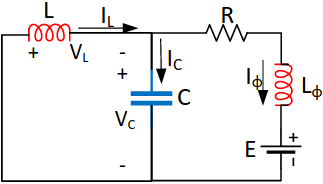
\includegraphics[width=0.3\textwidth]{Images/Phase_2}
\end{figure}

\noindent\\
Για την επίλυση του συστήματος  και πάλι χρησιμοποιούνται οι ίδιες μεταβλητές εισόδου και εξόδου με την Φ1 καθώς και οι ίδιες σχέσεις συστήματος (σχέσεις (\ref{x_dot}), (\ref{y})).  Αντίστοιχα οι πίνακες A, B, C και D προκύπτουν εφαρμόζοντας νόμο τάσεων του Kirchhoff:
\begin{align}
	\begin{rcases}
		V_L = L \cdot \frac{dI_L(t)}{dt} = - V_o\\
		V_c = V_o
	\end{rcases} V_L = -V_c &\xRightarrow{} \frac{dI_L(t)}{dt} = -\frac{1}{L} \cdot V_c\\
	V_c - I_{\Phi} \cdot R - \frac{dIL_{\Phi}}{dt} \cdot L_{\Phi} - E = 0 &\xRightarrow{}  \frac{dIL_{\Phi}}{dt} = -\frac{R}{L_{\Phi}} \cdot I_{\Phi} + \frac{1}{L_{\Phi}} \cdot V_c - \frac{1}{L_{\Phi}} \cdot E
\end{align}

και	 νόμο ρευμάτων του Kirchhoff:
\begin{equation}
	I_L = I_c + I_{\Phi} \xRightarrow{} \frac{dV_c}{dt} \cdot C = I_L - I_{\Phi} \xRightarrow{} \frac{dV_c}{dt} = \frac{1}{C} \cdot I_L - \frac{1}{C} \cdot I_{\Phi}
\end{equation}

\noindent
Επιλύοντας τις σχέσεις σε μορφή πινάκων σύμφωνα με τις σχέσεις (\ref{x_dot}) και (\ref{y}) προκύπτουν τα εξής συστήματα:
\begin{equation*}
	\overbrace{
		\frac{d}{dt} 
		\begin{bmatrix}
			I_L\\
			I_{\Phi}\\
			V_c
		\end{bmatrix}
	}^{\dot{X}}
	=
	\overbrace{
		\begin{bmatrix}
			0 		& 					0 			 & -\frac{1}{L}\\
			0       & -\frac{R}{L_{\Phi}} & \frac{1}{L_{\Phi}}\\
			\frac{1}{C}  & 		   -\frac{1}{C}      & 				0
		\end{bmatrix}
	}^A
	\cdot
	\overbrace{
		\begin{bmatrix}
			I_L\\
			I_{\Phi}\\
			V_c
		\end{bmatrix}
	}^X
	+ 	
	\overbrace{
		\begin{bmatrix}
			0  			&	    			0 			\\
			0           &  -\frac{1}{L_{\Phi}}\\
			0		    & 		  			0
		\end{bmatrix}
	}^B
	\cdot
	\overbrace{
		\begin{bmatrix}
			V_s\\
			E		
		\end{bmatrix}
	}^U
\end{equation*} 

\begin{equation*}
	\underbrace{
		\begin{bmatrix}
			I_L\\
			I_{\Phi}\\
			V_c
		\end{bmatrix}
	}_Y
	=
	\underbrace{
		\begin{bmatrix}
			1 & 0 & 0\\
			0 & 1 & 0\\
			0 & 0 & 1
		\end{bmatrix}
	}_C
	\cdot
	\underbrace{
		\begin{bmatrix}
			I_L\\
			I_{\Phi}\\
			V_c
		\end{bmatrix}
	}_X
	+ 
	\underbrace{	
		\begin{bmatrix}
			0 & 0 \\
			0 & 0 \\
			0 & 0
		\end{bmatrix}
	}_D
	\cdot
	\underbrace{
		\begin{bmatrix}
			V_s\\
			E		
		\end{bmatrix}
	}_U
\end{equation*}
\noindent\\\\
Τέλος όσον αφορά το ρεύμα πηνίου καθώς και την διακύμανσή του, σύμφωνα με την θεωρία προκύπτουν ίσα με:
\begin{align}
	I_L &= \frac{- V_o}{L}t \label{I_L_2}\\	
	\Delta I_L &= \frac{- V_o}{L} \cdot (1 - D) \cdot T \label{DI_L_2}
\end{align}

\subsection{Ελεγχόμενος μετατροπέας υποβιβασμού}